% --------------------------------------------------------------
% This is all preamble stuff that you don't have to worry about.
% Head down to where it says "Start here"
% --------------------------------------------------------------
 
\documentclass[12pt]{article}
 
\usepackage[margin=1in]{geometry} 
\usepackage{amsmath,amsthm,amssymb}
\usepackage{xcolor}
\usepackage{listings}
\usepackage{graphicx}
\usepackage{hyperref}
\usepackage{listings}
\usepackage{stackengine}
\usepackage{array}
\graphicspath{{/home/arpit/Desktop/iitd/sem_7/COL334/projects/Getting-To-Know-Network-Traffic/img}}

\newcommand{\N}{\mathbb{N}}
\newcommand{\Z}{\mathbb{Z}}
 
\newenvironment{theorem}[2][Theorem]{\begin{trivlist}
\item[\hskip \labelsep {\bfseries #1}\hskip \labelsep {\bfseries #2.}]}{\end{trivlist}}
\newenvironment{lemma}[2][Lemma]{\begin{trivlist}
\item[\hskip \labelsep {\bfseries #1}\hskip \labelsep {\bfseries #2.}]}{\end{trivlist}}
\newenvironment{exercise}[2][Exercise]{\begin{trivlist}
\item[\hskip \labelsep {\bfseries #1}\hskip \labelsep {\bfseries #2.}]}{\end{trivlist}}
\newenvironment{problem}[2][Problem]{\begin{trivlist}
\item[\hskip \labelsep {\bfseries #1}\hskip \labelsep {\bfseries #2.}]}{\end{trivlist}}
\newenvironment{question}[2][Question]{\begin{trivlist}
\item[\hskip \labelsep {\bfseries #1}\hskip \labelsep {\bfseries #2.}]}{\end{trivlist}}
\newenvironment{corollary}[2][Corollary]{\begin{trivlist}
\item[\hskip \labelsep {\bfseries #1}\hskip \labelsep {\bfseries #2.}]}{\end{trivlist}}

\newenvironment{solution}{\begin{proof}[Solution]}{\end{proof}}
\definecolor{codegreen}{rgb}{0,0.6,0}
\definecolor{codegray}{rgb}{0.5,0.5,0.5}
\definecolor{codepurple}{rgb}{0.58,0,0.82}
\definecolor{backcolour}{rgb}{0.95,0.95,0.92}

\lstdefinestyle{mystyle}{
    backgroundcolor=\color{backcolour},   
    commentstyle=\color{codegreen},
    keywordstyle=\color{magenta},
    numberstyle=\tiny\color{codegray},
    stringstyle=\color{codepurple},
    basicstyle=\ttfamily\footnotesize,
    breakatwhitespace=false,         
    breaklines=true,                 
    captionpos=b,                    
    keepspaces=true,                 
    numbers=left,                    
    numbersep=5pt,                  
    showspaces=false,                
    showstringspaces=false,
    showtabs=false,                  
    tabsize=2
}
\lstset{style=mystyle}
\begin{document}
 
% --------------------------------------------------------------
%                         Start here
% --------------------------------------------------------------
 
\title{Assignment 1: Getting to Know Network Traffic}
\author{Arpit Prasad\\ 
COL334: Computer Network}

\maketitle
\section{Measurement Tools}

\subsection{ping}

\begin{figure}[h!]
    \centering
    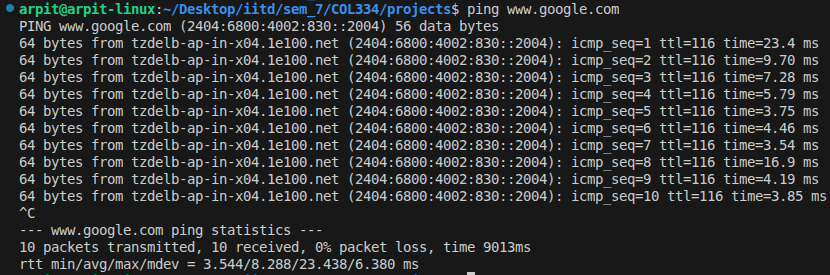
\includegraphics[width=0.8\textwidth]{google_ping.png}
    \caption{Ten Pings to www.google.com}
\end{figure}

\begin{figure}[h!]
    \centering
    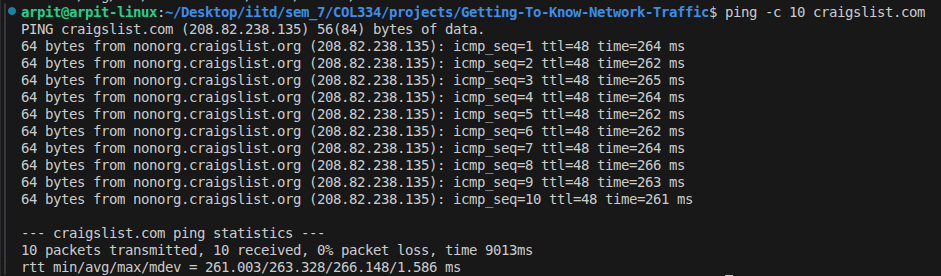
\includegraphics[width=0.8\textwidth]{craigslist_ping.png}
    \caption{Ten Pings to craigslist.com}
\end{figure}

\begin{enumerate}
    \item \textbf{Protocols Used}: Ping uses ICMP protocol which is on top of the IP protocol. It uses the Echo Request packet to the destination host and recieves Echo Reply packet from the same. It sits on the third layer of the protocol stack.
    \item \textbf{Latency}:
    \begin{enumerate}
        \item \textbf{Avg Latency of Craigslist}: 263.328 ms
        \item \textbf{Avg Latency of Google}: 6.832 ms
        \item Google's host has \textbf{smaller RTT} than Craigslist
        \item \textbf{Reason for different latencies of websites}:
        \begin{enumerate}
            \item Google has more number of hosts than Craigslist, which splits newtwork traffic
            % \item Physical distance to Google's host is lesser than Craigslist's host, hence reaching the destination host earlier. (Craigslist has a host in San Fransico, whereas, Google's hosts are distributed all across the world, as well as in India, hence smaller RTT)
        \end{enumerate}
        \item \textbf{Reason for differnt latencies across pings for same website}:
        \begin{enumerate}
            \item Length of Queue for service at destination host is not constant in time and varies according to the number of user who requested for service before, we place any request (queueing of packets, at the host)
            \item Network congestion is not constant, hence each switch in the network may not have same number of packets it has to route across differnt time
            \item Differnt routes may be taken for different pings leading to different distances and hence latencies
        \end{enumerate}
    \end{enumerate}
    \item using IPv6 for both websites
    \begin{figure}[h!]
        \centering
        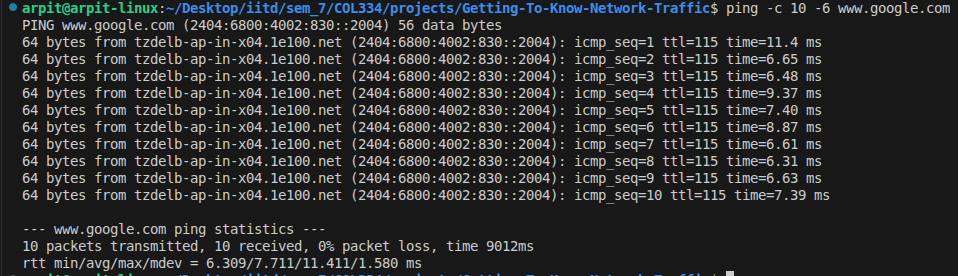
\includegraphics[width=0.8\textwidth]{google_ping_6.png}
        \caption{Ten Pings to www.google.com using IPv6}
    \end{figure}
    \begin{figure}[h!]
        \centering
        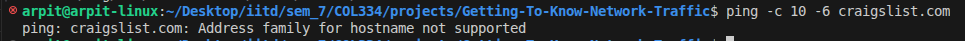
\includegraphics[width=0.8\textwidth]{craigslist_ping_6.png}
        \caption{Error when pinging craigslist.com}
    \end{figure}
    \begin{enumerate}
        \item How to force IPv6: pass a flag -6 to force ping to follow IPv6
        \item Result: IPv6 was supported by Google's host but not by Craigslist's host
        \item Why $ping -6$ Failed for Craigslist's host: Since IPv6 worked for Google's host, implies that my computer and Google's host both support IPv6. If a failure of Address Family support has occured it must have occured on Craigslist's server. This implies Craigslist's server does not support IPv6 addresses
    \end{enumerate}
    \item Max size of the packets
    \begin{table}[h!]
        \centering
        \caption{Max Size of Data Transmitted from Ping, practically obtained by experiment}
        \begin{tabular}{|c|c|c|c|}
            \hline
            Host & Max Message Size & ICMP Header Size & Max Total Size \\
            \hline
            www.google.com & 1462 bytes & 8 bytes & 1470 bytes \\
            craigslist.com & 283 bytes & 28 bytes & 311 bytes \\
            \hline
        \end{tabular}
    \end{table}
    \begin{enumerate}
        \item Reason of Limit to Size: The network interfaces have a Maximum Transmission Unit for precautions (not to overload a server or a network device, which would disallow the timely servicing of all packets), that limit the packet size. Hence the bottleneck in the path is the device with the smallest MTU 
        \item The packet size may also be limited by the OS
        \item For IPv6 over ethernet networks is limited ideally to 1500 bytes, but Table 1 shows what was practically achieved 
        \item The difference between practical and ideal may be caused by a network device through which the packet was routed has smaller MTU.
        \item To send a larger packet size, the packet must be fragmented
    \end{enumerate}
\end{enumerate}

\subsection{traceroute}
\begin{enumerate}
    \item IPv4 Address for www.google.com : 172.217.26.36
    \item IPv4 Address for craigslist.com : 208.82.238.135
\end{enumerate}

\begin{figure}[h!]
    \centering
    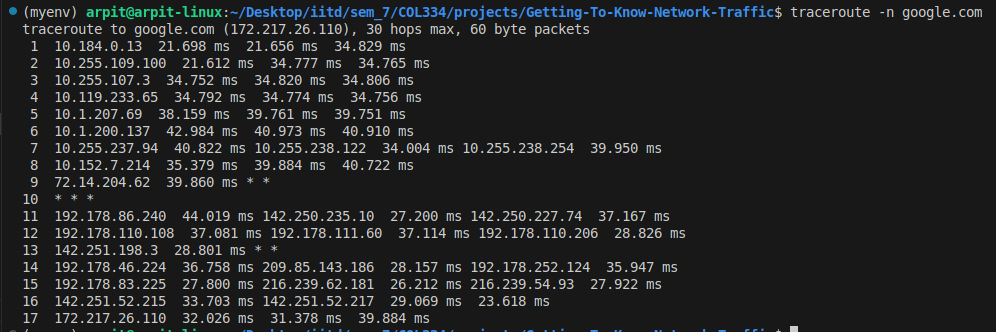
\includegraphics[width=0.8\textwidth]{google_tr.png}
    \caption{Trace Route of sending packet to www.google.com}
\end{figure}

\begin{figure}[h!]
    \centering
    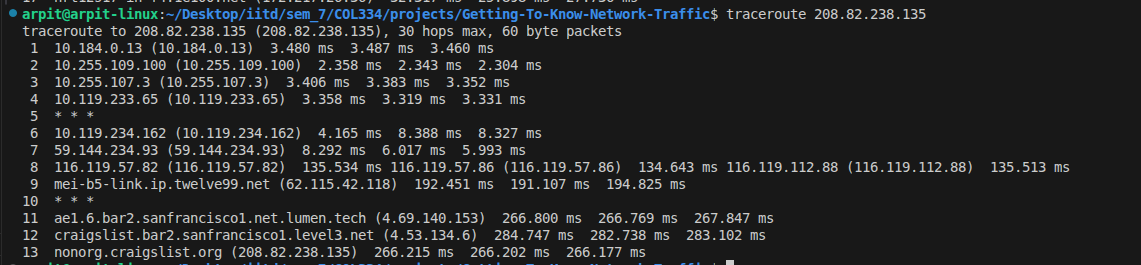
\includegraphics[width=0.8\textwidth]{craigslist_tr.png}
    \caption{Trace Route of sending packet to craigslist.com}
\end{figure}
\renewcommand{\labelenumi}{\Alph{enumi}}
\begin{enumerate}
    \item Number of Hops:
    \begin{table}[h!]
        \centering
        \caption{Number of Hops for Websites}
        \begin{tabular}{|c|c|}
            \hline
            Host & Number of Hops \\
            \hline
            www.google.com & 17 \\
            craigslist.com & 13 \\
            \hline
        \end{tabular}
    \end{table}
    \begin{figure}[h!]
        \centering
        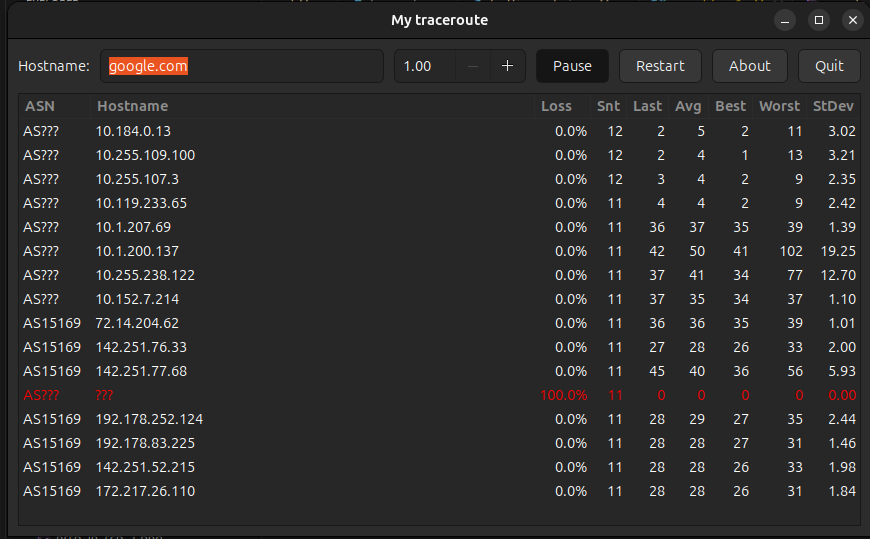
\includegraphics[width=0.8\textwidth]{google_asn.png}
        \caption{Autonomous System Number for each IP Address in the trace route of www.google.com (produces using mtr)}
    \end{figure}
    \begin{figure}[h!]
        \centering
        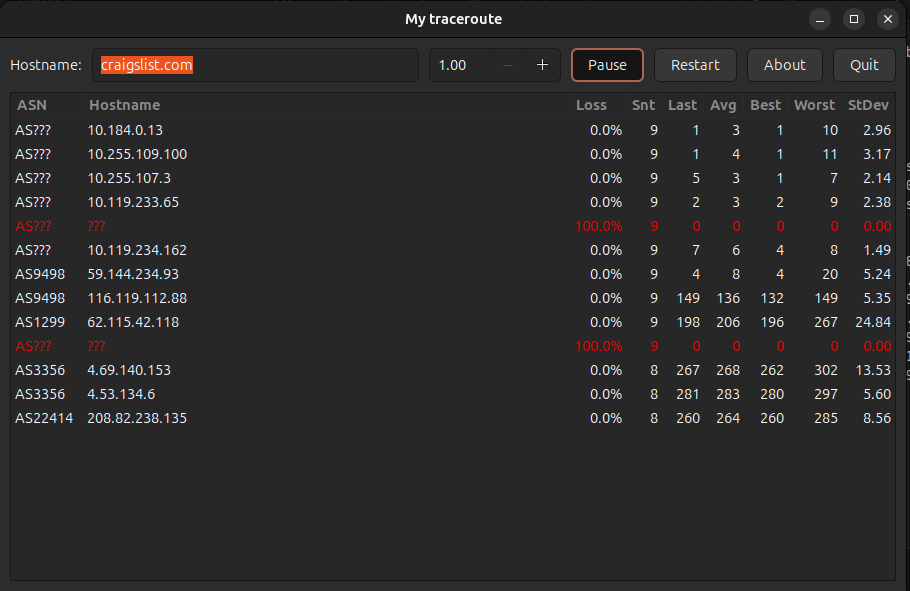
\includegraphics[width=0.8\textwidth]{craigslist_asn.png}
        \caption{Autonomous System Number for each IP Address in the trace route of craigslist.com (produces using mtr)}
    \end{figure}
    \item Explanation for "*": Some servers do not cater to traceroute packets, for security reasons and traffic control, hence do not send the Time Exceeded packet back to the source and hence, we do not have information about this node. This is represented in the traceroute by "*"
    \item Multiple IP Addresses for the same Hop Count: $traceroute$ sends three packets for each hop. The three packets may opt for independent routes, depending on the congestion of the network. traceroute lists all the unique ip addresses of the nodes encountered by the three packets
    \item The following table lists the IP Addresses and their correspoding RTTs and Geolocations
    \begin{table}[h!]
        \centering
        \caption{IP Addresses and their GeoLocations for www.google.com}
        \resizebox{\linewidth}{!}{
        \begin{tabular}{|c|c|>{\centering\arraybackslash}m{0.5\textwidth}|>{\centering\arraybackslash}m{0.5\textwidth}|>{\centering\arraybackslash}m{0.5\textwidth}|c|}
            \hline
            Sl No & IP Address & DNS & DNS Geolocation & Maxmind Geolocation & RTT (ms) \\
            \hline
            1 & 10.194.0.1 & NA & NA & NA 6.100 \\
            2 & 10.254.238.1 & NA & NA & NA & 6.087 \\
            3 & 10.255.107.3 & NA & NA & NA & 21.154 \\
            4 & 10.119.233.65 & NA & NA & NA & 21.147 \\
            5 & 10.1.207.69 & NA & NA & NA & 37.188 \\
            6 & 10.1.200.137 & NA & NA & NA & 50.264 \\
            7 & 10.255.237.94 & NA & NA & NA & 115.352 \\
            8 & 10.152.7.214 & NA & NA & NA & 215.550 \\
            9 & 72.14.204.62 & NA & NA & United States (US), North America & 215.512 \\
            10 & NA & NA & NA & NA \\
            11 & 142.250.214.102 & NA & NA & United States (US), North America & 186.456 \\
            12 & 142.251.77.68 & NA & NA & United States (US), North America & 151.676 \\
            13 & 142.251.197.253 & NA & NA & United States (US), North America & 33.512 \\
            14 & 142.251.247.50 & NA & NA & United States (US), North America & 36.570 \\
            15 & 192.178.83.215 & NA & NA & United States (US), North America & 59.573 \\
            16 & 142.251.49.115 & NA & NA & United States (US), North America & 45.122 \\
            17 & 172.217.26.36 & nrt12s17-in-f4.1e100.net or nrt12s17-in-f36.1e100.net or tzdelb-ap-in-f4.1e100.net & Narita, Japan, Tanzania & United States (US), North America & 48.186 \\
            \hline
        \end{tabular} }
    \end{table}
    \begin{table}[h!]
        \centering
        \caption{IP Addresses and their GeoLocations for craigslist.com}
        \resizebox{\linewidth}{!}{
        \begin{tabular}{|c|c|c| >{\centering\arraybackslash}m{0.5\textwidth} | >{\centering\arraybackslash}m{0.5\textwidth} |c|c|}
            \hline
            Sl No & IP Address & DNS & DNS Geolocation & Maxmind Geolocation & RTT (ms) \\
            \hline
            1 & 10.184.0.13 & NA & NA & NA & 685.733 \\
            2 & 10.255.109.100 & NA & NA & NA & 685.597 \\
            3 & 10.255.107.3 & NA & NA & NA & 685.551 \\
            4 & 10.119.233.65 & NA & NA & NA & 685.507 \\
            5 & * & NA & NA & NA & * \\
            6 & 10.119.234.162 & NA & NA & NA & 685.376 \\
            7 & 59.144.234.93 & NA & NA & Bengaluru, Karnataka, India & 5.715 \\
            8 & 116.119.112.88 & NA & NA & India & 138.551 \\
            9 & 62.115.42.118 & mei-b5-link.ip.twelve99.net & Meridian, Mississippi, USA & France & 197.050 \\
            10 & * & NA & NA & NA & * \\
            11 & 4.69.140.153 & ae1.6.bar2.SanFrancisco1.net.lumen.tech & San Francisco, California, United States (US), North America & United States, North America & 268.401 \\
            12 & 4.53.134.6 & CRAIGSLIST.bar2.SanFrancisco1.Level3.net & San Francisco, California, United States (US), North America & San Francisco, California, United States (US), North America & 270.387 \\
            13 & 208.82.238.135 & nonorg.craigslist.org & San Francisco, California, United States (US), North America & San Francisco, California, United States (US), North America & 259.620 \\
            \hline
        \end{tabular}}
    \end{table}

    \begin{enumerate}
        \item For the case of www.google.com, most of the network devices that relay the packet are private and hence no information is obtained about them. However we observe a delta in 9th hop, therefore we can assume that the packet has crossed the country.
        \item For craigslist.com : The bigger deltas are observed when there is a change in country. For eg., from Table 4, we observe that upto Bangalore the RTT was 5.77 ms but as the relay proceeded to the US, the RTT becomes signficanly higher, 197.05 ms. 
    \end{enumerate}

    Hence the data intuitively makes sense.
    
    \item Three Tier Architecture:
    \begin{enumerate}
        \item craigslist.com : Here we observe the three tier architecture clearly. Since first the packet travels from Delhi to Bangalore (which is a 2nd tier ISP transfer), then the exchange is observed from Bangalore to France and France to San Fransico which are a 1st Tier ISP Transfer. Finally 2nd and 3rd tier transfers occur for the packet to reach craigslist.com server
        \item www.google.com : Here, we do not observe the three tier architecture clearly. Most of the transfers are through private ip addresses. From RTTs we can conclude some of these transfers are in India and the rest directly in the US. This also occurs when a collection of network devices are considered as private network and do not disclose thier actual IP Address. Google might use these private networks for data transfers, for security reasons, such as avoiding data leaks. TODO
    \end{enumerate}
\end{enumerate}

\section{Network Traffic Collection and Analysis}

\subsection{Traffic Capture}
\renewcommand{\labelenumi}{\Alph{enumi}}
\begin{enumerate}
    \item Time taken for the DNS request-response to comlete: Query Time = 0.5815 and Response Time is 0.6966, time taken is \textbf{0.115}
    \item HTTP
    \begin{enumerate}
        \item Number of HTTP Requests = 364 (fitler used: $http.request$)
        \item How webpages are structured: The webpage is very modular. All images are loaded one by one on the website indicating completion of download.
        \item How browsers render complex pages with multiple images and files: They render the images one at a time, since from the packet information it can be observed different times of completion of the downloads
    \end{enumerate}
    \item TCP Connection
    \begin{enumerate}
        \item Number of TCP Connections = 31 (filter used: $tcp.flags.syn == 1 and tcp.flags.ack == 0$)
        \item Number of HTTP Conbnections==Number of TCP Connections: No, they are generally not equal, however they are related. In one TCP Connection multiple HTTP requests can be made.
        \item Content Object Fetch over same TCP Connection: Yes, some contents get fetched over the same TCP Connection. This can be supported from the fact that HTTP transfer are made with HTTP/1.1, which implies sustained TCP Connection for multiple HTTP transfers. This was verified using the filter $tcp.flags.syn==1 and tcp.flags.ack==0$ and the we checked the upstream flow. This showed multiple HTTP/1.1 transfers in one TCP Connection
        \begin{figure}[h!]
            \centering
            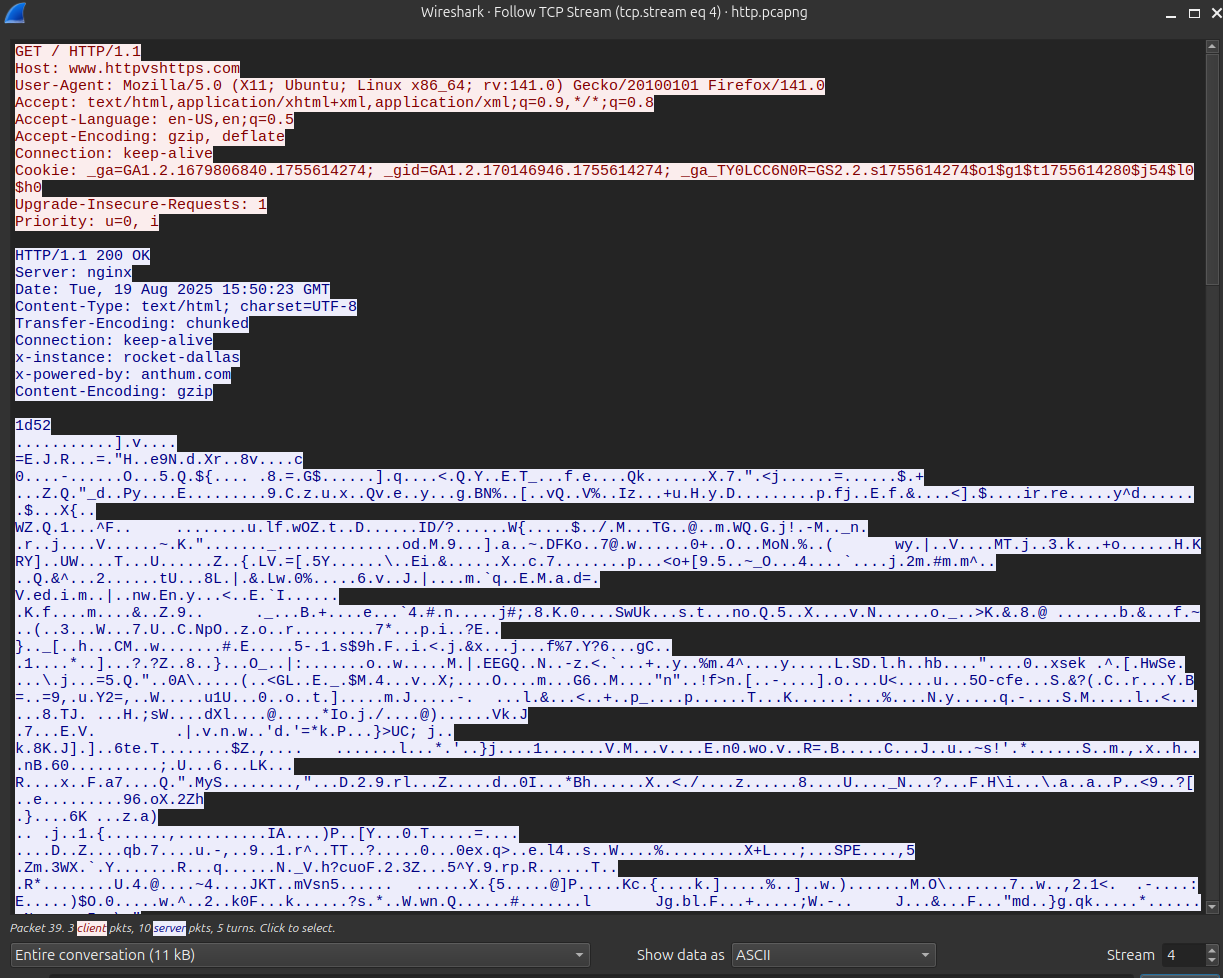
\includegraphics[width=0.8\textwidth]{http_in_tcp.png}
        \end{figure}
    \end{enumerate}
    \item HTTPs packet trace
    \begin{enumerate}
        \item http traffic there? No, there is no HTTP Traffic
        \item content transfer of HTTP and JavaScript files? and why?: There is no content tranfer of HTTP and JavaScript. HTTPs is secured data transfer, therefor the file content is encrypted and hence not visible without the key to the file. This is the reason why wireshark does not show this content
        \item dns traffic: Yes, DNS Traffic is present. DNS is required for look ups to convert web addresses to their correspoding IP Addresses.
        \item number of tcp connections logged = 25
        \item Number of HTTP Conbnectinos==Number of TCP Connections: They are not equal in this case. However the HTTPS case has smaller number of TCP Connections. A potential reason is multiplexing, allowing many HTTPS request to be sent simultaneously.
    \end{enumerate}
\end{enumerate}

\subsection{Performance Analysis}
\begin{enumerate}
    \item[E] HTTP vs HTTPs
    \begin{enumerate}
        \item comparision of time taken for downloads: HTPP::17.132s and HTTPs::1.614 (93\% faster than HTTP)
        \item Observation from the plots: 
        \begin{enumerate}
            \item The download plot for https.pcap has significant throughput for download in comparision to that for http.pcap. Since the amount of data downloaded is the same, hence if the time of download reduces, this implies throughput increases.
            \item This can also be referred from the RTT plot. Since RTT is very small for most of the times that are plotted, we can infer the small download time in the case of htpps.pcap and larger download time in the case of http.pcap
        \end{enumerate}
         
        \begin{figure}[h!]
            \centering
            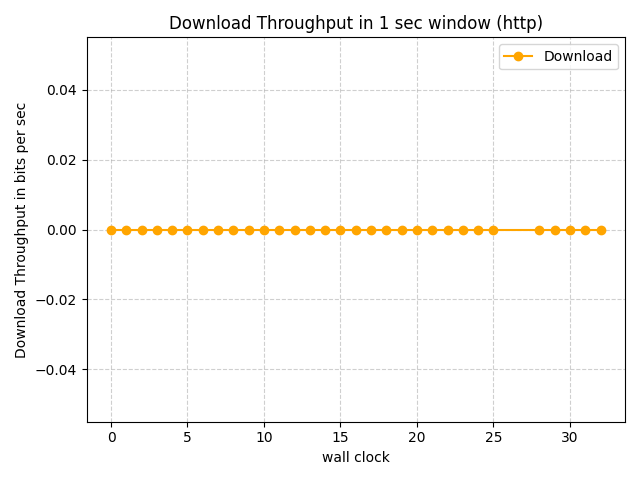
\includegraphics[width=0.8\textwidth]{down_throughput.png}
            \caption{Download Throughput using http.pcap}
        \end{figure}
        \begin{figure}[h!]
            \centering
            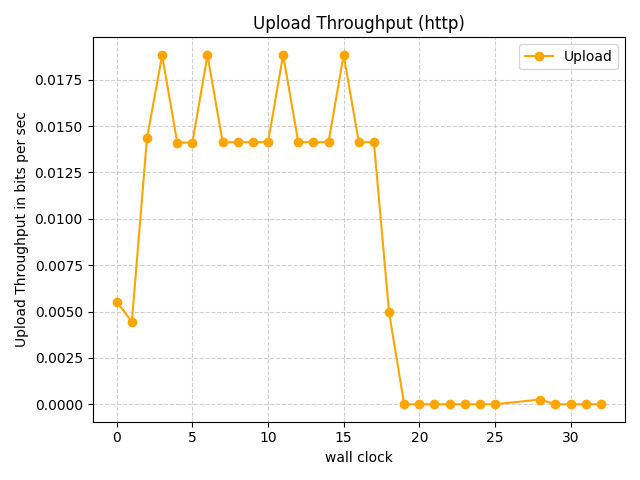
\includegraphics[width=0.8\textwidth]{up_throughput.png}
            \caption{Upload Throughput using http.pcap}
        \end{figure}
        \begin{figure}[h!]
            \centering
            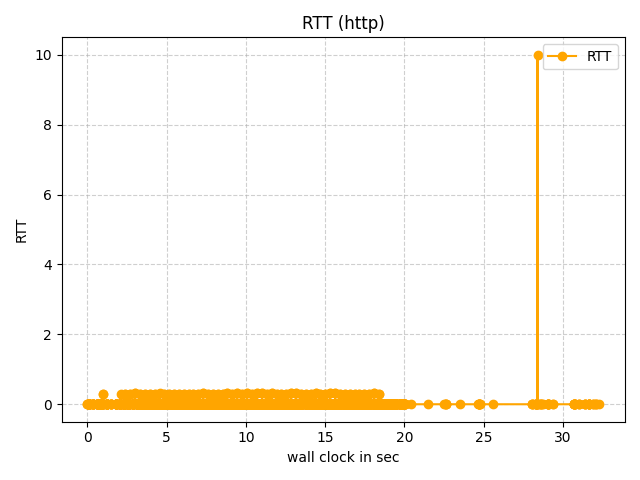
\includegraphics[width=0.8\textwidth]{rtt.png}
            \caption{RTT using http.pcap}
        \end{figure}
        \begin{figure}[h!]
            \centering
            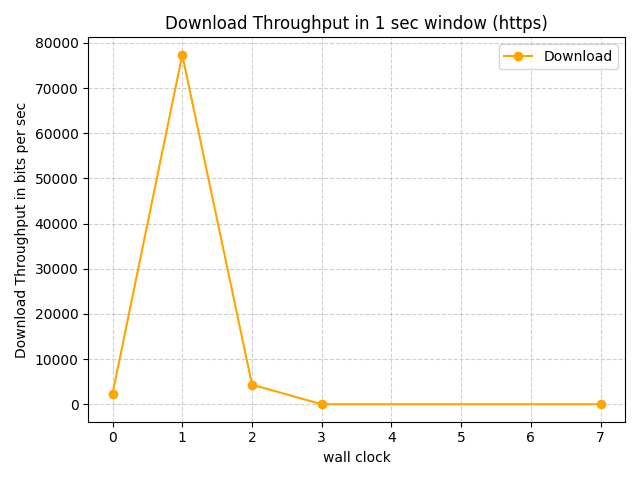
\includegraphics[width=0.8\textwidth]{down_throughput_s.png}
            \caption{Download Throughput using https.pcap}
        \end{figure}
        \begin{figure}[h!]
            \centering
            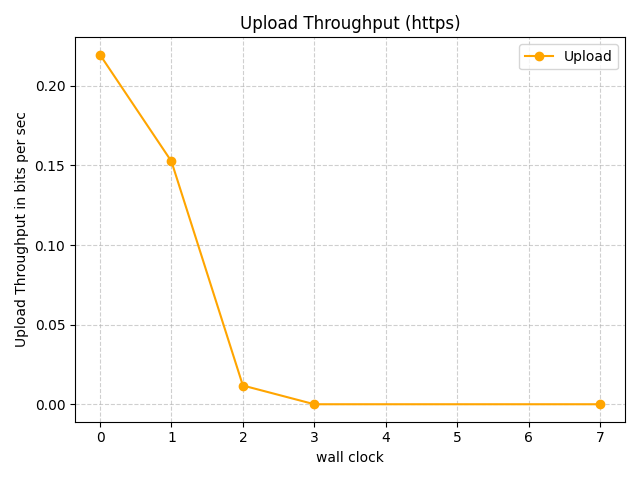
\includegraphics[width=0.8\textwidth]{up_throughput_s.png}
            \caption{Upload Throughput using https.pcap}
        \end{figure}
        \begin{figure}[h!]
            \centering
            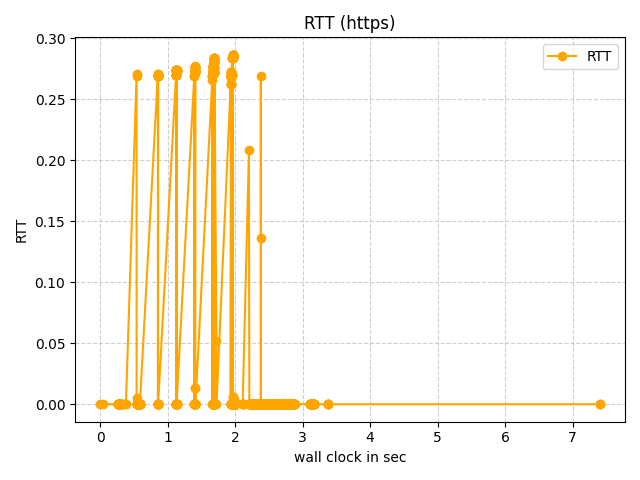
\includegraphics[width=0.8\textwidth]{rtt_s.png}
            \caption{RTT using http.pcap}
        \end{figure}
    \end{enumerate}
    
\end{enumerate}
% --------------------------------------------------------------
%     You don't have to mess with anything below this line.
% --------------------------------------------------------------

\end{document}
